\documentclass[12pt,a4paper]{article}
\usepackage[english]{babel}
\usepackage[utf8]{inputenc}
\usepackage[margin=1in]{geometry}
\usepackage{natbib,graphicx,amsmath,amssymb,subfigure,float,bm}
\pagestyle{headings}
\usepackage{blindtext}
\title{\textbf{Winter Storm Friedhelm} - A Case Study}
\date{\today}
\author{Jacob Perez}
\setlength{\parindent}{0em}
\setlength{\parskip}{2.5mm}
\begin{document}
\maketitle
\begin{abstract}
    Winter storm Friedhelm was a mid-latitude cyclone that struck the country of Scotland in December of 2011. In this work, we present a detailed analysis based on quasi-geostrophic theory, of different dynamic and thermodynamic variables to describe the life cycle of this cyclone. 
\end{abstract}
\tableofcontents
\section{Introduction}
On December 8th of 2011 an extratropical cyclone named Friedhelm, shown here in figure \ref{friedhelm}, struck the coast of Scotland bringing with it hurricane force winds and mountains of snow leading to disruptions and damages to peoples everyday lives. The work presented here investigates the dynamics behind the formation of the cyclone and how it progressed across the Atlantic and over the UK. We take assess the dynamics of the cyclone following quasi-geostrophic theory to start making links to vertical motion, thermal wind relation, and taking a potential vorticity (PV) perspective as well. 
\begin{figure}[H]
    \centering
    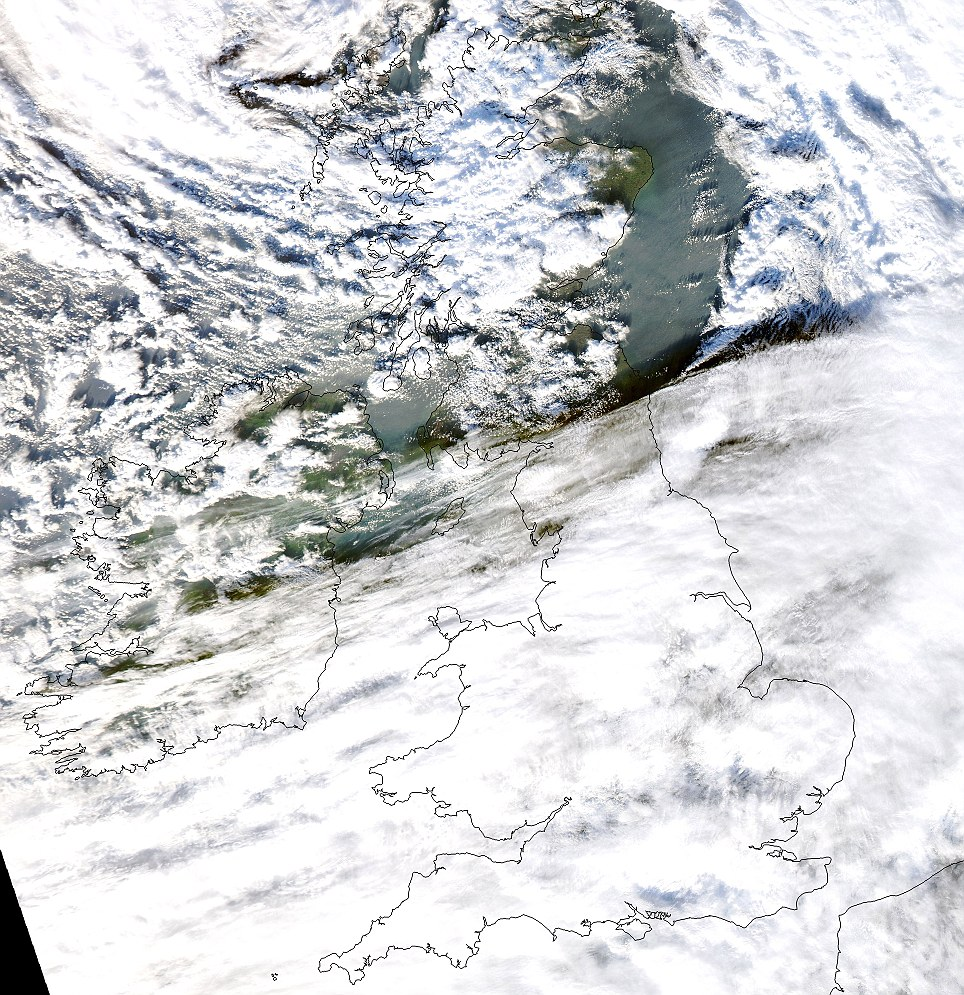
\includegraphics[width=0.5\textwidth]{friedhelm.jpg}
    \caption{A satellite image of the cyclone as it sat over the UK.}
    \label{friedhelm}
\end{figure}
\section{Methods}
In this work, we use the ERA-Interim reanalysis dataset to conduct the analysis. The ERA-interim dataset is observational data that has been assimilated onto a 0.25$^o \times$0.25$^o$ grid. The data will be analysed following dynamical theories of weather forecasting focusing on quasi-geostrophic theories shown to us in the Dynamics of Weather systems course at the University of Leeds and from textbooks by \cite{Hoskins2013} and \cite{Holton2015} The data presented in the plots shown here have been produced using Python. 
\section{Analysis}
\subsection{MSLP, Relative Vorticity and Wind Speed} \label{pvw}
From the ERA-interim data, we begin by looking at the mean surface level pressure (MSLP). In figure \ref{MSLP} we have the MSLP on the day of the storm. We can see that a low-pressure system at 00:00 begins to develop off the west coast of Scotland and at 12:00 the low-pressure region sits on top of Scotland and moving towards the east later on in the day. This indicates that we have warming in this region meaning we have high winds and warmer air, indicating vertical motion. Taking the winds close to the surface and in the middle of the troposphere we take the wind speed at the 850hPa and 500hPa levels, these are shown in figure \ref{windspeeds}. At the 850hPa level, we see high winds in the 30-40 ms$^{-1}$ range with circulation patterns emerging with the winds in this region. The moving higher up in the atmosphere to the 500hPa we see that we have much stronger winds reaching speeds of 60ms$^{-1}$ in a similar position to that of the circulation regions seen much closer to the surface. Looking at figure \ref{Q} we can also see a distinct increase in humidity across the day moving with the low pressure region and over the UK.
\begin{figure}[H]
    \centering
    \subfigure[00:00]{\includegraphics[width=0.45\textwidth]{plots/ERA_interim_MSLP_20111208_0000.png}} 
    \subfigure[06:00]{\includegraphics[width=0.45\textwidth]{plots/ERA_interim_MSLP_20111208_0600.png}} 
    \subfigure[12:00]{\includegraphics[width=0.45\textwidth]{plots/ERA_interim_MSLP_20111208_1200.png}}
    \subfigure[18:00]{\includegraphics[width=0.45\textwidth]{plots/ERA_interim_MSLP_20111208_1800.png}}
    \caption{Development of a surface low over the west coast of Scotland on the 8th of December.}
    \label{MSLP}
\end{figure}
\begin{figure}[H]
\centering
    \centering
    \subfigure[850hPa]{\includegraphics[width=0.45\textwidth]{plots/ERA_interim_Windspeed_20111208_1200_850hPa.png}} 
    \subfigure[500hPa]{\includegraphics[width=0.45\textwidth]{plots/ERA_interim_Windspeed_20111208_1200_500hPa.png}} 
    \caption{Windspeed contours with wind vectors $u$ and $v$ on the 8th of December at 12:00.}
    \label{windspeeds}
\end{figure}
\begin{figure}[H]
    \centering
    \subfigure[00:00]{\includegraphics[width=0.45\textwidth]{plots/ERA_interim_specific_humidity20111208_0000_850hPa.png}} 
    \subfigure[06:00]{\includegraphics[width=0.45\textwidth]{plots/ERA_interim_specific_humidity20111208_0600_850hPa.png}} 
    \subfigure[12:00]{\includegraphics[width=0.45\textwidth]{plots/ERA_interim_specific_humidity20111208_1200_850hPa.png}}
    \subfigure[18:00]{\includegraphics[width=0.45\textwidth]{plots/ERA_interim_specific_humidity20111208_1800_850hPa.png}}
    \caption{Development of a surface low over the west coast of Scotland on the 8th of December.}
    \label{Q}
\end{figure}
We now wish to analyse the vertical motion further by considering the relative vorticity. Starting with the relative vorticity in figure \ref{relative vorticity} where we have plotted the relative vorticity taken at 500hPa, the reason being this is the level of a vorticity maximum and best choice to assess ridges and troughs. In this plot, see an exact overlap with positive values of relative vorticity and the low pressure regions seen in the MSLP, starting at around 20$^o$W and moving eastward. These two are related as positive values of relative vorticity indicate anti-cyclonic motion meaning we have vertical motion. The vertical motion is linked to following equation,
\begin{equation}
    \nabla_H \cdot\bm{U} = -\frac{\partial w}{\partial z}
    \label{divergenceeqn}
\end{equation}
which states that horizontal divergence of the wind leads to a decreasing vertical velocity with height and a horizontal convergence leads to an increasing vertical velocity with height. Figure \ref{divergence} shows the divergence and the vertical velocity on the 8th of December at 12:00, this was chosen due to the large positive relative vorticity occurring. In figure \ref{divergence} we see that at the 850hPa level we have a weakly negative divergence, indicating converging winds and a stronger positive divergence indicating diverging winds over Scotland. Comparing this with the vertical velocity at the same level, we see a dipole of vertical velocity forming negative vertical velocity corresponding to ascending air and positive meaning descending air understood from equation \eqref{divergenceeqn}.   
Comparing this to the same plots at 250hPa we see the that that at upper levels we have the opposite as to what was occurring at the surface i.e. where we had convergence at the surface we have divergence at the higher levels and vice versa, relating to back to equation \eqref{divergenceeqn}. 
\begin{figure}[H]
    \centering
        \centering
        \subfigure[00:00]{\includegraphics[width=0.45\textwidth]{plots/ERA_interim_Relative_Vorticity_20111208_0000_500hPa.png}} 
        \subfigure[06:00]{\includegraphics[width=0.45\textwidth]{plots/ERA_interim_Relative_Vorticity_20111208_0600_500hPa.png}} 
        \subfigure[12:00]{\includegraphics[width=0.45\textwidth]{plots/ERA_interim_Relative_Vorticity_20111208_1200_500hPa.png}} 
        \subfigure[18:00]{\includegraphics[width=0.45\textwidth]{plots/ERA_interim_Relative_Vorticity_20111208_1800_500hPa.png}} 
        \caption{Relative vorticity contours at 500hPa on the 8th of December.}
        \label{relative vorticity}
\end{figure}
\begin{figure}[H]
    \centering
        \subfigure[850hPa]{\includegraphics[width=0.45\textwidth]{plots/ERA_interim_Divergence_20111208_1200_850hPa.png}} 
        \subfigure[250hPa]{\includegraphics[width=0.45\textwidth]{plots/ERA_interim_Divergence_20111208_1200_250hPa.png}} 
        \subfigure[850hPa]{\includegraphics[width=0.45\textwidth]{plots/ERA_interim_Vertical_velocity_20111208_1200_850hPa.png}}
        \subfigure[250hPa]{\includegraphics[width=0.45\textwidth]{plots/ERA_interim_Vertical_velocity_20111208_1200_250hPa.png}}
        \caption{The divergence and vertical velocity at 850hPa and 250hPa on the 8th of December at 12:00.}
        \label{divergence}
\end{figure}
This can be seen further in a plot of the cross-section shown in figure \ref{verticalcross} which is the vertical velocity at 5$^o$W at 12:00. Here we can see a strong vertical velocity occurring at 60$^o$W and weakening slightly as you move poleward. Regions of strong vertical velocity are also regions with high precipitation and rain fall. In figures \ref{cloudcontents600} and \ref{cloudcontents1200} we have horizontal and vertical plots of the cloud liquid and ice water content at 06:00 and at 12:00. We can see a distinct increase of surface level water content as the cloud ice content moves across Scotland. This indicates a warming within the region of high water content as the water content increases as the ice content begins to decrease. The increase in water content vertically is due to the higher humidity in the area that we saw in figure \ref{Q}.
\begin{figure}
\centering
\subfigure[5$^o$W]{\includegraphics[width=0.45\textwidth]{plots/ERA_interim_CLWC_Cross_Section20111208_0600_Longitude_-5.png}}
\subfigure[5$^o$W]{\includegraphics[width=0.45\textwidth]{plots/ERA_interim_CIWC_Cross_Section20111208_0600_Longitude_-5.png}}
\subfigure[850hPa]{\includegraphics[width=0.45\textwidth]{plots/ERA_interim_CLWC_20111208_0600_850hPa.png}}
\subfigure[500hPa]{\includegraphics[width=0.45\textwidth]{plots/ERA_interim_CLIC_20111208_0600_500hPa.png}}
\label{cloudcontents600}
\caption{Cloud water (a,c) and ice (b,d) contents at 06:00 on the 8th of December}
\end{figure}

\begin{figure}
\centering
\subfigure[0$^o$]{\includegraphics[width=0.45\textwidth]{plots/ERA_interim_CLWC_Cross_Section20111208_1200_Longitude_0.png}}
\subfigure[0$^o$]{\includegraphics[width=0.45\textwidth]{plots/ERA_interim_CIWC_Cross_Section20111208_1200_Longitude_0.png}}
\subfigure[850hPa]{\includegraphics[width=0.45\textwidth]{plots/ERA_interim_CLWC_20111208_1200_850hPa.png}}
\subfigure[500hPa]{\includegraphics[width=0.45\textwidth]{plots/ERA_interim_CLIC_20111208_1200_500hPa.png}}
\caption{Cloud water (a,c) and ice (b,d) contents at 12:00 on the 8th of December}
\label{cloudcontents1200}
\end{figure}

To better understand the intensity of the vertical motion we can compare the vertical motion of the wind speed at the centre of the respective regions of high relative vorticity as it moves across Scotland. In figure \ref{vertical windspeed} we show a cross-section of the vertical wind speed at each of these locations. It can be seen that at 5$^o$W, corresponding to 12:00 on the 8th of December, we have high windspeeds located at around 500hPa reaching speeds of 40ms$^{-1}$ and higher. We can also compare this to the previous 12 hours and see that the intensity of the vorticity at the surface is also increasing, as we start to see much higher windspeed values as the positive vorticity sits over Scotland. 
\begin{figure}[H]
    \centering
    \includegraphics[width=0.75\textwidth]{plots/ERA_interim_w_Cross_Section20111208_1200_Longitude_-5.png}
    \caption{Vertical cross section of the vertical velocity at 5$^o$W at 12:00.}
    \label{verticalcross}
\end{figure}
\begin{figure}[H]
        \centering
            \centering
            \subfigure[20$^o$W]{\includegraphics[width=0.45\textwidth]{plots/ERA_interim_Windspeed_Cross_Section20111208_0000_Longitude_-20.png}} 
            \subfigure[14$^o$W]{\includegraphics[width=0.45\textwidth]{plots/ERA_interim_Windspeed_Cross_Section20111208_0600_Longitude_-14.png}} 
            \subfigure[5$^o$W]{\includegraphics[width=0.45\textwidth]{plots/ERA_interim_Windspeed_Cross_Section20111208_1200_Longitude_-5.png}} 
            \subfigure[0$^o$]{\includegraphics[width=0.45\textwidth]{plots/ERA_interim_Windspeed_Cross_Section20111208_1800_Longitude_0.png}} 
            \caption{Vertical windspeed at the points of maximum relative vorticity corresponding to the surface low.}
            \label{vertical windspeed}
\end{figure}
\subsection{Variations in Temperature and the Geostrophic Wind}
We now want to see what an event that may have caused this system to form. In the mid-latitudes it is common to see that vertical motion as intense as is seen in the formation of storms is created by baroclinic events, usually linked to rapidly changing temperatures triggering vertical motion. So with that let us consider the potential temperature in the days prior to the storm. Shown in figure \ref{potential temperature} is a contour plot of the potential temperature at 850hPa layered with a solid contour being the MSLP. What we can see is that in the region of a strong meridional temperature gradient located about 15-20$^o$W we have the compressing MSLP contours, corresponding to our surface low that we discussed in section \ref{pvw}. Furthermore, we can see that the centre of the surface low follows the the most intense region of the meridional gradient of the potential temperature. What we are seeing at this point is the formation of a cold front due to a steep temperature gradient forming which leads to a large vertical shear due the thermal wind relation which is,
\begin{equation}
\bm{v}_T = \frac{\partial \bm{v}_g}{\partial z} = \frac{g}{f\overline{\theta}}\bm{k}\times\nabla_H\theta
\end{equation}
where $\bm{v}_g$ is the geostrophic wind and $\theta$ is the potential temperature. This we can see in the in figure \ref{geostrophic wind} where we have geostrophic wind vectors at 850hPa, 500hPa and 250hPa to see the strength of the geostrophic wind as we move up through the atmosphere over this temperature gradient. We can see that in the presence of this temperature gradient this creates an imbalance to the geostrophic wind, as the vectors begin to deviate away from the contours of the geopotential height and this carries through all the way up to the tropopause height. We also see that the vectors turn anticlockwise with height, indicating that there is cold advection occurring based on the thermal wind relation. 

Since geostrophic winds are based on a horizontal balance between the Coriolis force and the pressure gradients, by looking at the ageostrophic winds we will see that they are the strongest where the the temperature gradient is the strongest. This can be seen in figure \ref{ageostrophic wind} where we the ageostrophic wind vectors plotted against the potential temperature contours and we can see that the magnitude of these vectors matches the regions where the temperature gradient is the strongest. If we also consider the vertical cross section of the temperature shown in figure \ref{tempcross} shown here at the each longitude where the centre of the surface low is travelling, we can see a distinct maximum occurring approximately at 800hPa and this is moving with the surface low. In particular at 12:00 we see a strong vertical temperature gradient forming corresponding to the very fast winds that we have seen in figures \ref{geostrophic wind} and \ref{windspeeds}.
\begin{figure}[H]
    \centering
        \centering
        \subfigure[00:00]{\includegraphics[width=0.45\textwidth]{plots/ERA_interim_potential_temperature_20111208_0000_850hPa.png}}  
        \subfigure[06:00]{\includegraphics[width=0.45\textwidth]{plots/ERA_interim_potential_temperature_20111208_0600_850hPa.png}} 
        \subfigure[12:00]{\includegraphics[width=0.45\textwidth]{plots/ERA_interim_potential_temperature_20111208_1200_850hPa.png}}  
        \subfigure[18:00]{\includegraphics[width=0.45\textwidth]{plots/ERA_interim_potential_temperature_20111208_1800_850hPa.png}}  
        \caption{Potential temperature on December 8th at 850hPa with black contours for the MSLP.}
        \label{potential temperature}
\end{figure}
\begin{figure}[H]
    \centering
        \centering
        \subfigure[850hPa]{\includegraphics[width=0.45\textwidth]{plots/ERA_interim_Z_geostrophic_20111208_1200_850hPa.png}}  
        \subfigure[500hPa]{\includegraphics[width=0.45\textwidth]{plots/ERA_interim_Z_geostrophic_20111208_1200_500hPa.png}}  
        \subfigure[250hPa]{\includegraphics[width=0.45\textwidth]{plots/ERA_interim_Z_geostrophic_20111208_1200_250hPa.png}}  
        \caption{Geopotential height contours and geostrophic wind vectors at 12:00.}
        \label{geostrophic wind}
\end{figure}
\begin{figure}[H]
    \centering
        \centering
        \subfigure[850hPa]{\includegraphics[width=0.45\textwidth]{plots/ERA_interim_theta_ageostrophic_20111208_1200_850hPa.png}}  
        \subfigure[500hPa]{\includegraphics[width=0.45\textwidth]{plots/ERA_interim_theta_ageostrophic_20111208_1200_500hPa.png}}  
        \subfigure[250hPa]{\includegraphics[width=0.45\textwidth]{plots/ERA_interim_theta_ageostrophic_20111208_1200_250hPa.png}}  
        \caption{Geopotential height contours and ageostrophic wind vectors at 12:00.}
        \label{ageostrophic wind}
\end{figure}
\begin{figure}[H]
    \centering
        \centering
        \subfigure[$20^o$W]{\includegraphics[width=0.45\textwidth]{plots/ERA_interim_T_Cross_Section20111208_0000_Longitude_-20.png}}  
        \subfigure[$14^o$W]{\includegraphics[width=0.45\textwidth]{plots/ERA_interim_T_Cross_Section20111208_0600_Longitude_-14.png}}  
        \subfigure[$5^o$W]{\includegraphics[width=0.45\textwidth]{plots/ERA_interim_T_Cross_Section20111208_1200_Longitude_-5.png}}
        \caption{Temperature cross section positioned of position of the surface low seen in figure \ref{MSLP}.}
        \label{tempcross}
\end{figure}
\subsection{PV Perspective}
We now consider the potential vorticity (PV) as the variable leading to the development of the cyclone. By considering the vertical cross section of the PV over the, centred at $22.5^o$W as this is the region of the highest relative vorticity as seen in figure \ref{relative vorticity} we find that the tropopause begins to reach down in the atmosphere indicating a positive PV anomaly forming in this region, which can be seen in figure \ref{PV cross section}. 
\begin{figure}
    \includegraphics[width=\textwidth]{plots/ERA_interim_PV_Cross_Section20111208_0000_Longitude_-22.5.png}
    \label{PV cross section}
    \caption{Cross section of PV at longitude $22.5^o$W. The lowest point of the tropopause occurring at 500hPa at $50^o$N. }
\end{figure}
This PV blob can be seen as to be "squashing" the surrounding air around it and so in an attempt to conserve PV we expect to see rapid descent poleward of the anomaly and descent equatorward of it. By considering the $\bm{Q}$ vector we can assess the vertical motion further. The $\bm{Q}$ vector is defined as 
\begin{equation} 
\bm{Q} = \left(-\frac{R}{p}\frac{\partial \bm{v}_g}{\partial x}\cdot\nabla T, - \frac{R}{p}\frac{\partial \bm{v}_g}{\partial y}\cdot\nabla T\right)
\end{equation}
where $R$ is the gas constant for air, $p$ is the pressure level you are at and $T$ is the temperature. This vector describes how geostrophic motion can alter the buoyancy gradient. Further by considering $\nabla_H\cdot\bm{Q}$ we find that there is negative correlation between this and the vertical velocity. 
In figure \ref{divQ} we have a plot of the $\nabla_H\cdot\bm{Q}$ on the day of the storm with contours of the potential temperature both plotted at 850hPa. What we can see is the that we have rapidly ascending and descending air occurring at the sharpest points of the temperature gradient forming this overturning circulation as the storm progresses towards the UK. Comparing this to vertical velocity see in section \ref{pvw} we see that these two agree in the positions at which they occur in.
\begin{figure}[H]
    \centering
        \subfigure[00:00]{\includegraphics[width=0.45\textwidth]{plots/ERA_interim_divQ_20111208_0000_850hPa.png}}  
        \subfigure[06:00]{\includegraphics[width=0.45\textwidth]{plots/ERA_interim_divQ_20111208_0600_850hPa.png}} 
        \subfigure[12:00]{\includegraphics[width=0.45\textwidth]{plots/ERA_interim_divQ_20111208_1200_850hPa.png}} 
        \subfigure[18:00]{\includegraphics[width=0.45\textwidth]{plots/ERA_interim_divQ_20111208_1800_850hPa.png}} 
        \caption{Contour plots of $\nabla_H \cdot \bm{Q}$ with solid contours of the potential temperature on December 8th. }
        \label{divQ}
\end{figure}
\section{Conclusion}
In this work we have looked at the winter storm Friedhelm and used the ERA-interim reanalysis data to assess its development, using ideas from quasi-geostrophic theory, as it moved over and across the UK. From the data we were able to identify a distinct sea surface low that occurred on December 8th at 00:00 which became stronger throughout day, reaching its maximum at 12:00 over the coast of Scotland. Analysing various dynamical variables we found that within this low we had high humidity leading to high ice and water contents belonging to it. Further we found a strong meridional temperature gradient, corresponding to a high amount of vertical motion which was assessed further through considerations of horizontal wind divergence, vorticity analysis and the geostrophic and ageostrophic winds. Finally we looked at the PV perspective by diagnosing at positive PV anomaly occurring in at the tropopause and connecting this to an overturning circulation forming using the $\bm{Q}$ causing a cold front to form, this being the storm and tracking this over the day. 
\bibliography{references.bib}
\bibliographystyle{apa}
\end{document}

